\begin{frame}{Árvore de recursão}
    \metroset{block=fill}

    \only<1-2>{
        \begin{block}{Algoritmo de fibonacci}
            \footnotesize
            \inputminted{cpp}{codigos/fib.cpp}    
        \end{block}
    }


    \only<2->{
        \begin{figure}[h]
        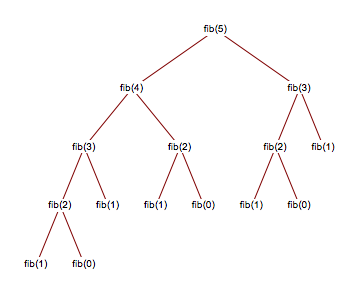
\includegraphics[scale=0.5]{fib.png}
        \end{figure}
    }

    \only<3->{
        A árvore completa tem $2^n$ passos, e o custo de cada nó é $O(1)$, então $T(n) = O(2^n)$.
    }

    \only<4->{
        {\bf Obs}. Uma análise da equação característica nos dá $T(n) = \Theta((1+\sqrt{5})/2)$.
    }

\end{frame}

